\clearpage
\section{Impulsive imaging}\seclab{Imag}

Source finding is performed by the script \verb!"Imaging.sh"! residing in the FlashFolder. The running of the script is controlled by \verb!"Imaging.in"!, which typically resembles


\begin{linenumbers}
\resetlinenumber
\tiny
\begin{verbatim}
&Parameters
 RunOption='Impulsive'
   Dual=.false.  ! Fix pulses in the even (Y-) and odd (X-) numbered dipoles at same source position.
! ChiSq_lim= 80 ! max value for chi^2 of a source for it to be stored (RMS=sqrt(chi^2)
! NoiseLevel=80. !  Any weaker sources will not be imaged.
! AntennaRange=100	! maximal distance of antennas to the reference antenna [km]
! PeaksPerChunk=500 !  Maximum number of sources searched for per chunk (of 0.3 ms).
! CalibratedOnly=.true. !  Use only antennas that have been calibrated.
! FullSourceSearch=.true. !  Perform without any preferred direction, otherwise take the sourceguess as a preference.
! Simulation=" " !  Run on simulated data from such files.
! EffAntNr_lim=0.8 !  minimal fraction of the total number of antennas for which the pulse is located.
! CCShapeCut_lim=0.6 !  Maximum ratio of the width of the cross correlation function by that of the self correlation.
! SearchRangeFallOff=4. !  Multiplier for the (parabolic) width of the pulse-search window.
! Sigma_AntT=3 !  Constant added to width of search window for pulses.
 Calibrations= "Calibrations201912042045.dat"
 BadAnt_SAI=   003065, 021078, 021079, 021093, 026030, 32016, 32017, 32048, 32049
               101045, 125029, 150065, 188051, 188094, 188095
 OutFileLabel="-s"
&end

C  1165 , -45500.  7700.   5300.0 , 101.7 300  !  StartTime_ms , (N,E,h), t_init [ms], t_fin [ms] (after start)
\end{verbatim}
\end{linenumbers}

While in imaging mode only very few parameters need to be specified and often the default settings will suffice.
\begin{enumerate*}
\item[2] \verb#"RunOption='Impulsive'"#: Run in impulsive imaging mode.
\item[3] \verb!" Dual=.false."!: The peaks in even and odd numbered antennas will be searched for independently.  \\
    \verb!" Dual=.true."!: In searching for the source locations the peak positions in both even- and odd-numbered antennas are used.
\item[4] \verb#"! ChiSq_lim= 80."#: Sources with a chi-square better than 80 will be stored.
\item[5] \verb#"! NoiseLevel = 80."#: The source location will be searched only for pulses with an amplitude in the reference antenna greater than 80.
\item[6] \verb#"! AntennaRange=100"#: All antennas within a distance of 100~km (the max possible) will from the reference antenna will be included in the calculations.
\item[7] \verb#"! PeaksPerChunk=500"#; Maximum number of sources searched for per chunk (of 0.3 ms).
\item[8] \verb#'! CalibratedOnly=.true.'#: Only antennas used in the calibration run will be used for imaging.
\item[9] \verb#"! FullSourceSearch=.true."#: Perform without any preferred direction, otherwise take the sourceguess as a preference.
\item[10] \verb#'! Simulation=" " '#: Run on simulated data from thus named files files, see \secref{?}.
\item[11] \verb#"! EffAntNr_lim=0.8" #:  minimal fraction of the total number of antennas for which the pulse is located.
\item[12] \verb#'! CCShapeCut_lim=0.6 '#:  Maximum ratio of the width of the cross correlation function by that of the self correlation.
\item[13] \verb#"! SearchRangeFallOff=4. " #:  Multiplier for the (parabolic) width of the pulse-search window.
\item[14] \verb#"! Sigma_AntT=3 " #:  Constant added to width of search window for pulses.
\item[15] \verb!' Calibrations = "Calibrations201912042045.dat"'!: The name of the calibration file created at the end of the time calibration procedure.
\item[16] \verb#" BadAnt_SAI=   003065, "#: The antenna SAI identifiers (see \secref{RFI-out}) of the antennas that do not have good data.
\item[18] \verb#' OutFileLabel="-s" '#: An additional label for the output files, including the list of sources.
\item[21] \verb#"C  1165 , -45500.  7700.   5300.0 , 101.7 300 "#: Specification of the starting time, approximate location of the flash, and the time frame where sources should be searched. If `S' is used instead of `C' (or space) the given time will correspond to the time at the indicated position.
\end{enumerate*}

The last line in the input specifies
\\1) The start time, $T_0=1165$  (in ms), of the flash. The output of the RFI-mitigation and also that of the Explore runs should give you a reasonable estimate of when the flash started.
\\2--4) The general direction towards the flash (N,E,h) in m.
\\5) The time after $T_0$ (in ms) to proceed with source finding. It may be negative.
\\6) The time after $T_0$ (in ms) to stop with source finding.

\subsection{details}

The results for the source locations are written to \verb!Srcs18-dblxxxx.csv! or otherwise the files \verb!Srcs18-oddxxxx.csv! and \verb!Srcs18-evenxxxx.csv! in the FlashFolder.
These .csv files are plain text files and contain some header lines with some general information followed by the specific data of the sources that are found and pass some very crude criteria. In particular $\chi^2<$\verb!ChiSq_lim!. The data for the sources is organized in columns where:
\\col1: Unique label composed from the chuck number (after $T_0$) and the pulse number in the chunk.
\\col2-4: distances northward, eastward, upward [m].
\\col5: Time at the source [s].
\\col6: $\chi^2$, if this had units, they would be [ns$^2$] .
\\col7-9: 1 std error in north, east, vertical direction [m].
\\col10: Number of antennas that have contributed to imaging this source.
\\col11: Total number of antennas for which data are available for this chunk.

See later sections for the details of the source-finding procedure including the criteria for excluding antennas.

\subsection{output}

The most important output is the list of source locations with their quality identifiers. Additionally a plot is made of the peak-finding statistics like shown in \figref{PeakStat}.

\begin{figure}[th]
\centering{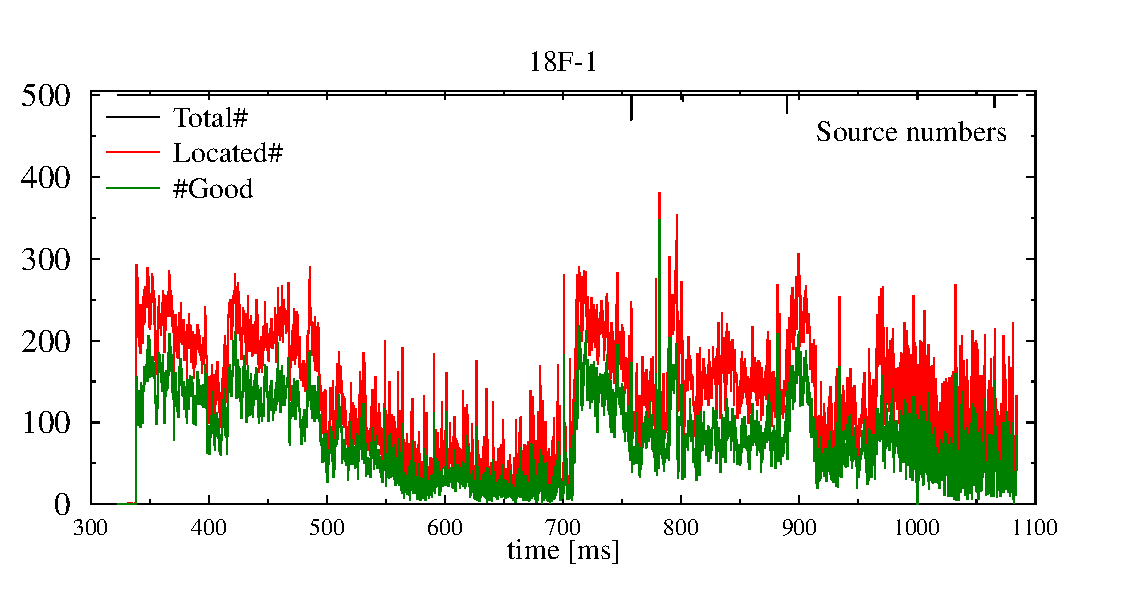
\includegraphics[bb=0cm 0cm 18.5cm 9.4cm,clip, width=0.49\textwidth]{Figs/PeakStats} }
%\centering{\includegraphics[ bb=1.0cm 2.4cm 24.5cm 25.7cm,clip, width=0.49\textwidth]{../Figs/SE20A7-NPMx_1HIntfSpecSel} }
	\caption{Statistics of the source-finding procedure for the impulsive imager. For each time frame the number of located sources is given with a chi-square below the maximum specified.}	 \figlab{PeakStat}
\end{figure}

\section{Plotting flashes}

Note: This section in obsolete by now since the utility \verb!FlashImage! is superseded by \verb!DataSelect! and discussed in \secref{DataSelect}.
The utility \verb!FlashImage! is depreciated and no longer maintained.

For plotting it is advised to use the script \verb!FlashImage.sh! that reads the input from \verb!FlashImage.in! specifying values for the quality indicators as well as the windows for which the source locations and timings will be plotted. The script \verb!FlashImage.bat! is for running under windows.

\begin{linenumbers}
\resetlinenumber
\small
\begin{verbatim}
 "Srcs18-evenS" 5. 2. 3.0 55   18D1e-i   -30.00 -27.  -7.5 -5.0  4.5 7.0  0. 30.  NoBox
 0.1 0.5 0.1      ""  1.  1.   1   0.5                                             ! MaxTrackDist[km], Wtr[0.5], TimeWin[ms^2]
======================================================
\end{verbatim}
\end{linenumbers}

The first line gives in order:
\\1) The name of the .csv file containing the sources data as created by an imaging run.
\\2) The cut $ \sigma_0^h $ on $\sigma{h}$
\\3) The height $h_0$. All sources higher than $h_0$ are plotted when  $\sigma{h} < \sigma_0^h$. Sources at lower altitudes $h$ will be plotted when $\sigma{h} < \sigma_0^h \times (h_0/h) $.
\\4) RMS cut value, in [ns].
\\5) $N_{ex}$, the maximum number of excluded stations.
\\6) naming of the .pdf file containing the image.
\\7 -- 14) limiting values for east, north, height (all in [km]) and time (in [ms] after $t_0$
\\15) if "NoBox" is specified, no high-lighting box will be drawn, otherwise the coordinates of the box will be read from the files for the specified plot.

The second line gives the parameters for calculating track that will be indicated in the image of the sources. In order:
\\1) maximal distance for a source to be removed from the track-head to be assigned to a track.
\\2) Weighting of additional points to determine the position of the track-head.
\\3) Width of gaussian time window to smooth the track.
\\4) Name of file containing predefined track.
\\5) Binning window for determining track statistics such as velocity.
\\6) Factor to scale height in the calculation of relative distances.
\\7) Integer. The maximum number of tracks to be generated.
\\8) Factor used to scale intensity-dependence of the size of the dots when plotting source positions.

\begin{figure}[th]
\centering{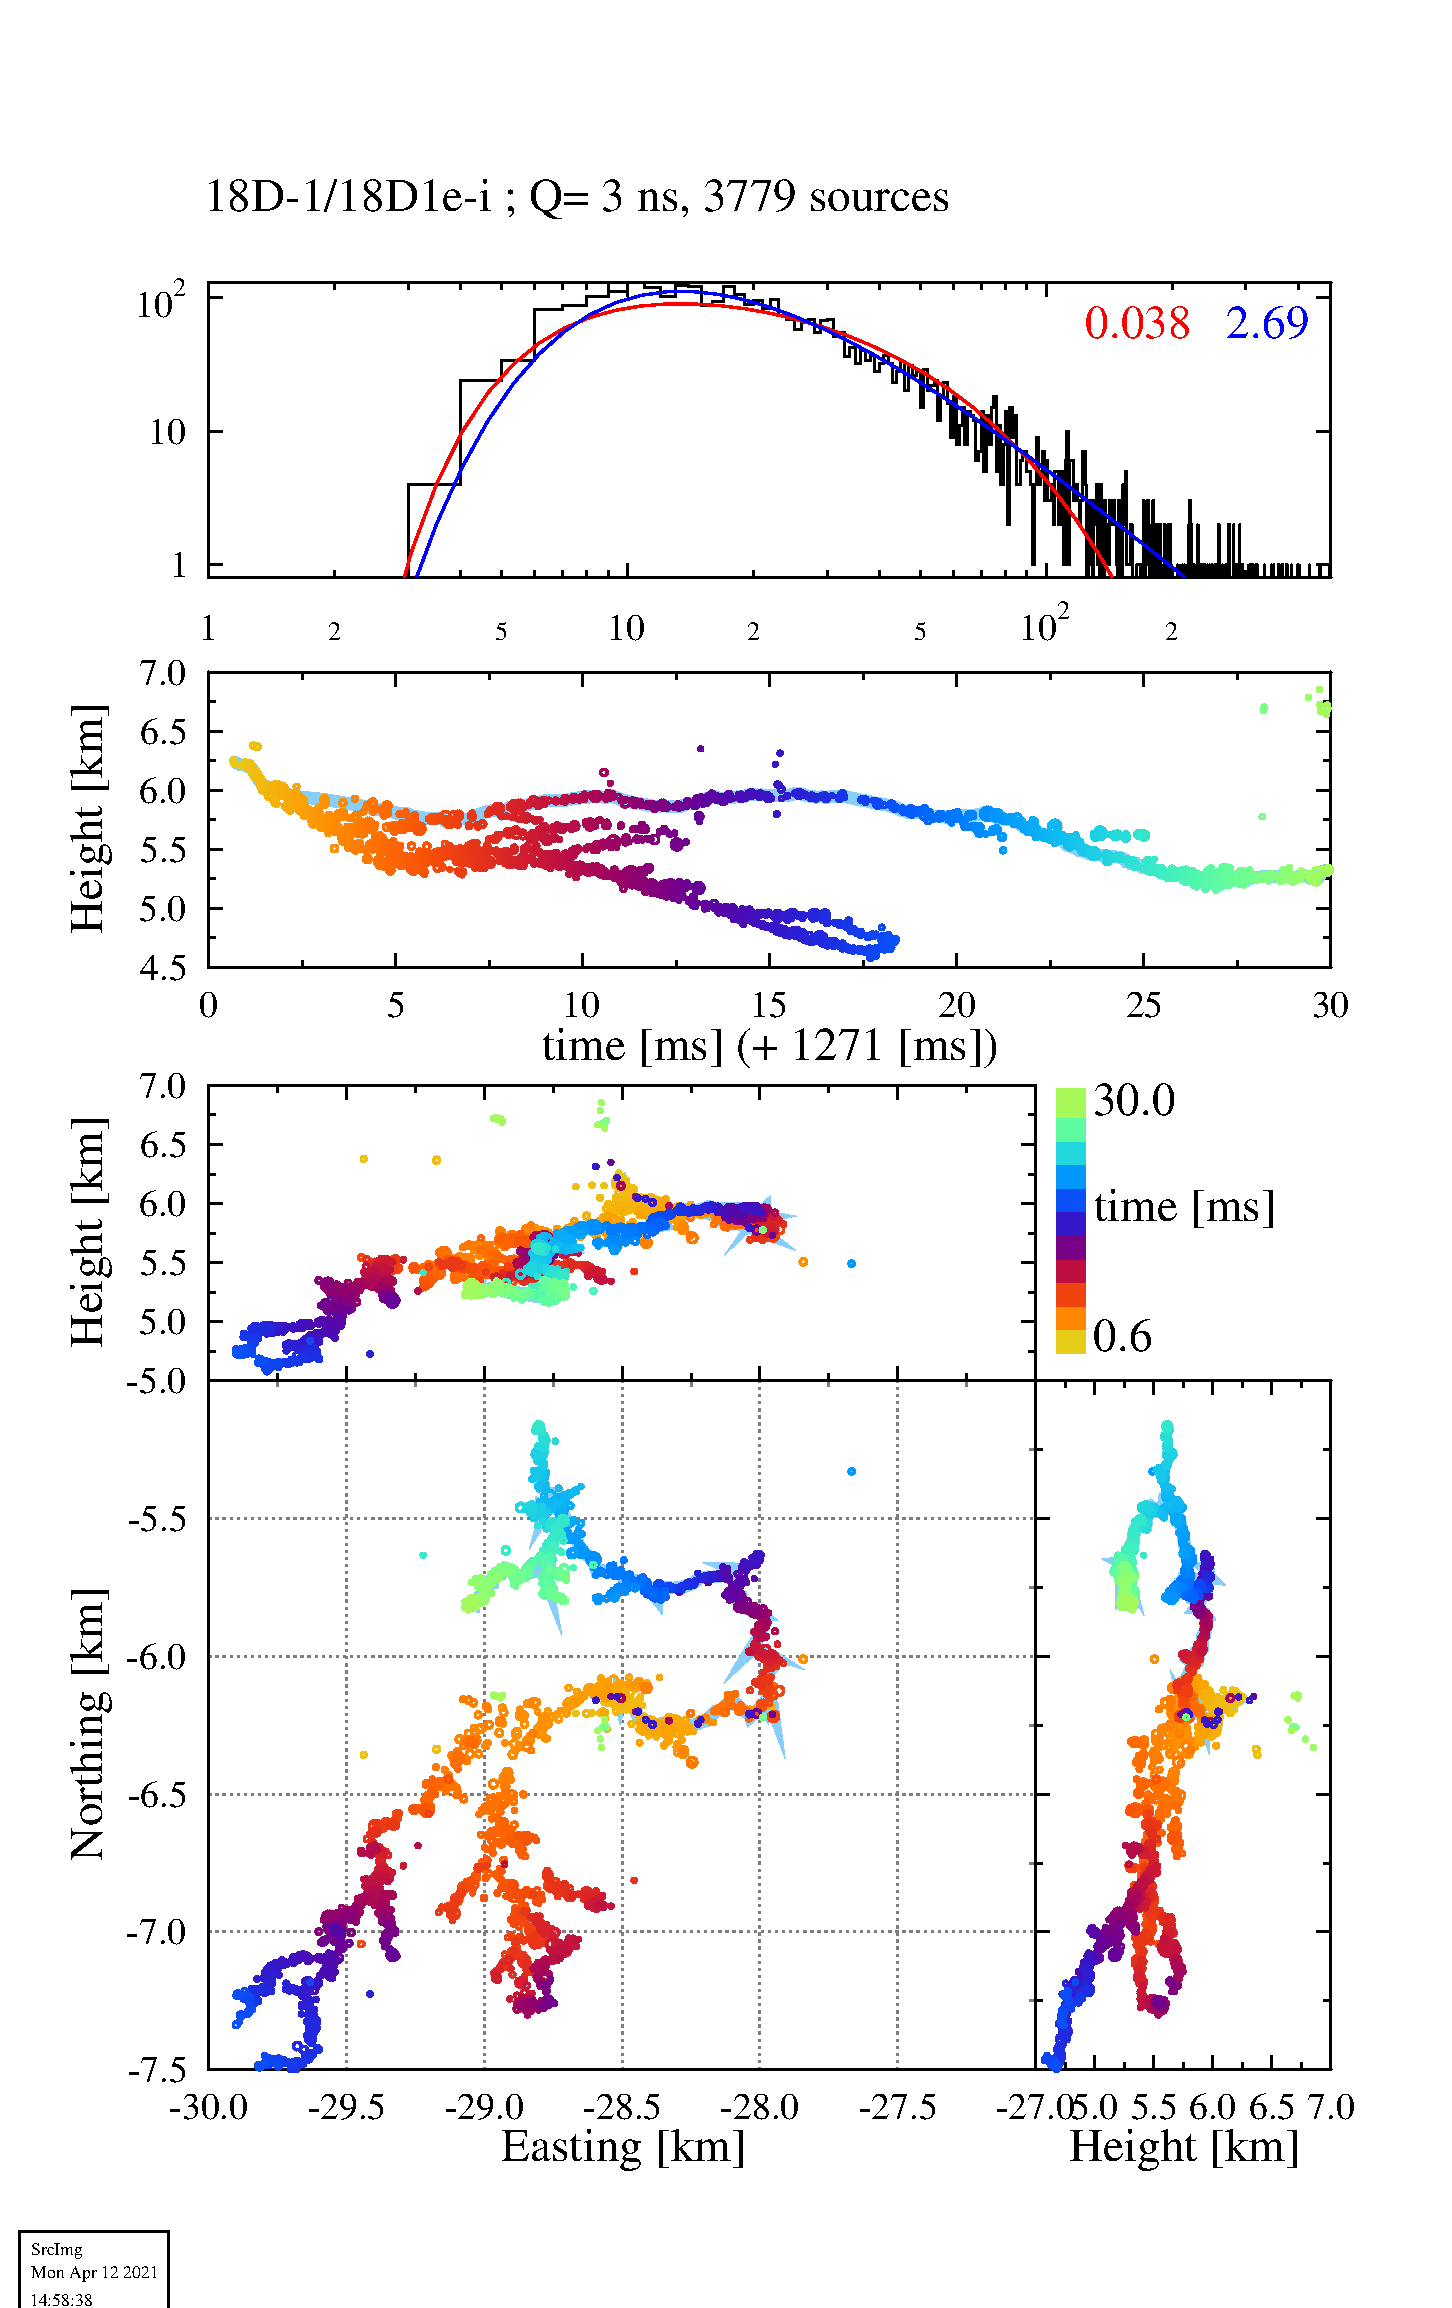
\includegraphics[width=0.49\textwidth]{Figs/Imp_18D1e-i} }
%\centering{\includegraphics[ bb=1.0cm 2.4cm 24.5cm 25.7cm,clip, width=0.49\textwidth]{../Figs/SE20A7-NPMx_1HIntfSpecSel} }
	\caption{Typical image for the Impulsive Imager as created by running ``FlashImage.bat". Light blue band is the reconstructed track (starting from the latest point and tracing back). Top panel give pulse power statistics where the modified exponential is plotted in red and the modified power law plotted in blue.}	 \figlab{ImpulsiveImg}
\end{figure}

The result is displayed in \figref{ImpulsiveImg} for the image of the flash for the selected area. The normalized pulse powers distributions $N(I)$ are fitted with a modified exponential,
\begin{equation}
N(I)= {\cal N}_e \,e^{-\alpha_e\,I-\gamma_e/I^2}\;, \eqlab{PowLaw}
\end{equation}
as well as with a modified powerlaw,
T\begin{equation}
N(I)= {\cal N} \,I^{-\alpha}  \,e^{-\gamma/I}\;, \eqlab{PowLaw}
\end{equation}
where $I$ is expressed in units of [GB]. The last factor, dependent on $\gamma$, suppresses the distribution at small amplitudes to good agreement with the data. The values for the fitted values for the normalization ${\cal N}$, the power $\alpha$, and the small-intensity suppression factor $\gamma$ are given in the output file (with extension .out).

\begin{figure}[th]
\centering{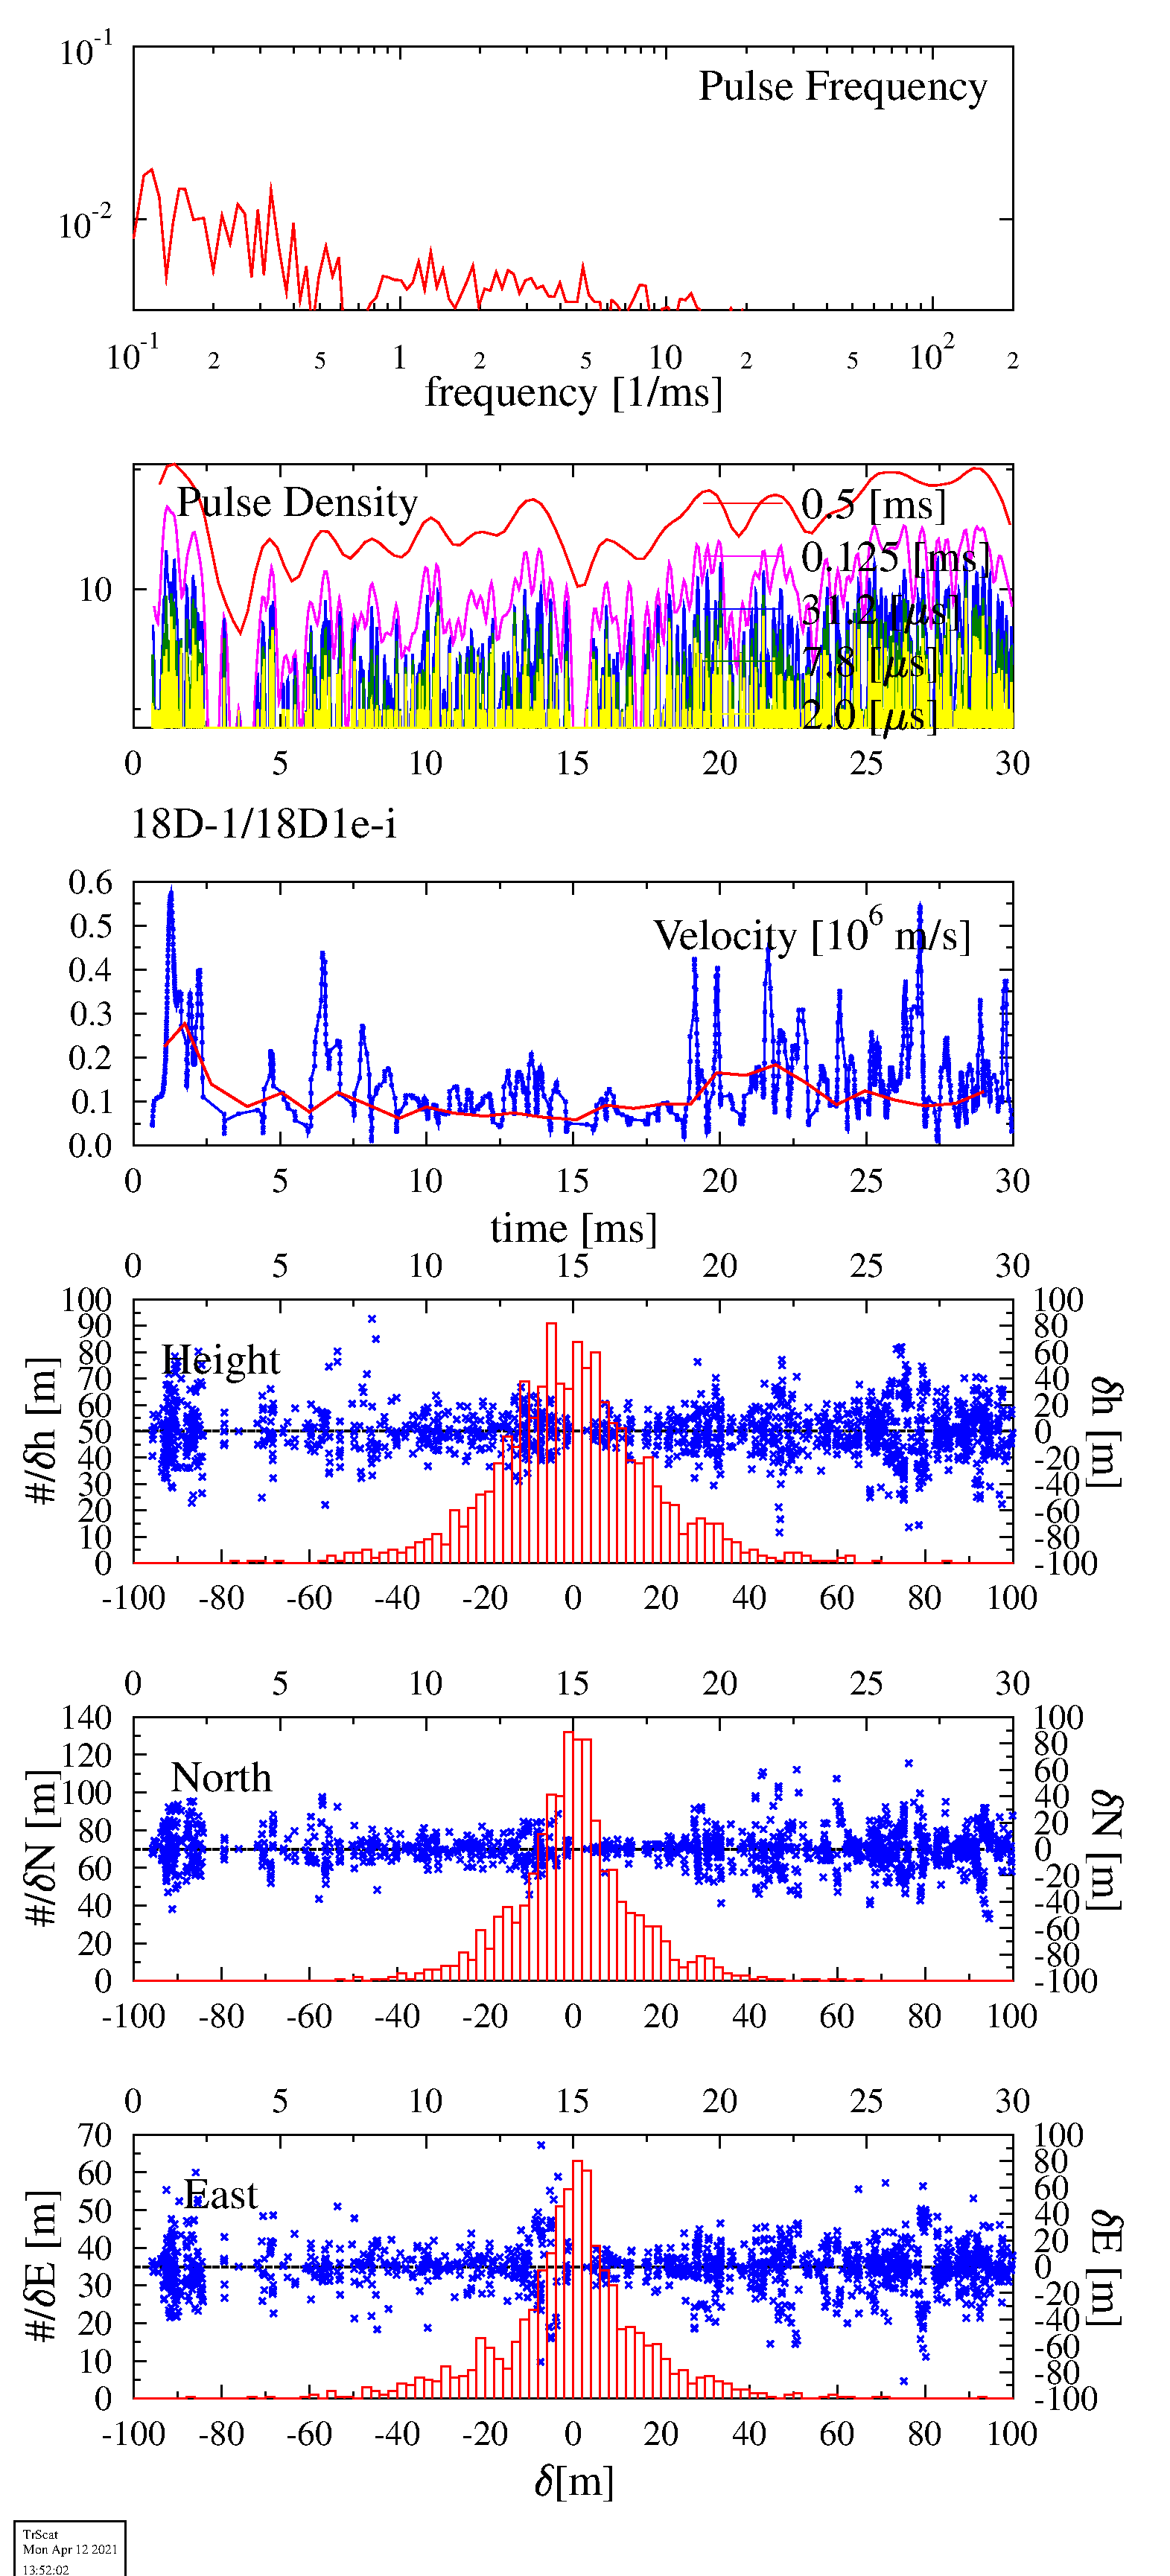
\includegraphics[ width=0.49\textwidth]{Figs/TrSc_18D1e-i} }
%\centering{\includegraphics[ bb=1.0cm 2.4cm 24.5cm 25.7cm,clip, width=0.49\textwidth]{../Figs/SE20A7-NPMx_1HIntfSpecSel} }
	\caption{Typical image for the Impulsive Imager when showing the statistics along a track.}	 \figlab{ImpulsiveTrack}
\end{figure}

If the 7th number on the second line in the input, ``FlashImage.in", is positive, a graph like \figref{ImpulsiveTrack} is made for each track. The second panel from the top shows the pulse density along the flash as function of time for various width of a gaussian smoothing function. The top panel shows the fourier decomposition of this plot. The third from the top gives the velocity along the track. The blue line for each source along the track, the red line for an average leader-tip location. The bottom three panels show the spread of the sources in the three directions from the propagating tip of the leader, in blue as a scatter plot v.s.\ time of the source (top and right scales), in red as a histogram (bottom and left scales).
\clearpage 